\subsection{Subset-sum}
Subset sum decision problem:
\begin{itemize}
	\item Instance: $n$ numbers $a_1, a_2, \cdots, a_n$ and a target $T$.
	\item Question: is there a subset $S$ of the indices such that $\sum_{i \in S} a_i = T$.
\end{itemize}

subset sum problem is in NP. Suppose you are given a YES-instance $\langle (a_1, a_2, \cdots, a_n), T \rangle$. Then a certificate showing it is a YES-instance would be that subset of numbers which add up to $T$. We could check the certificate by adding up $(a_1, a_2, \cdots, a_n)$ to see if the sum is $T$.

We prove that subset sum is NP-complete by a complicated reduction from 3-SAT. Let $\varphi$ be a 3-SAT instance with $n$ variables and $m$ clauses. We create a subset sum instance with $2n + 2m$ numbers, each with $n+m$ digits!

Every row suppose to be one number. The first a few digits are the variable columns and the last few digits are the clauses columns. So there are $n + m$ columns in total. 

\begin{figure}[H]
	\centering
	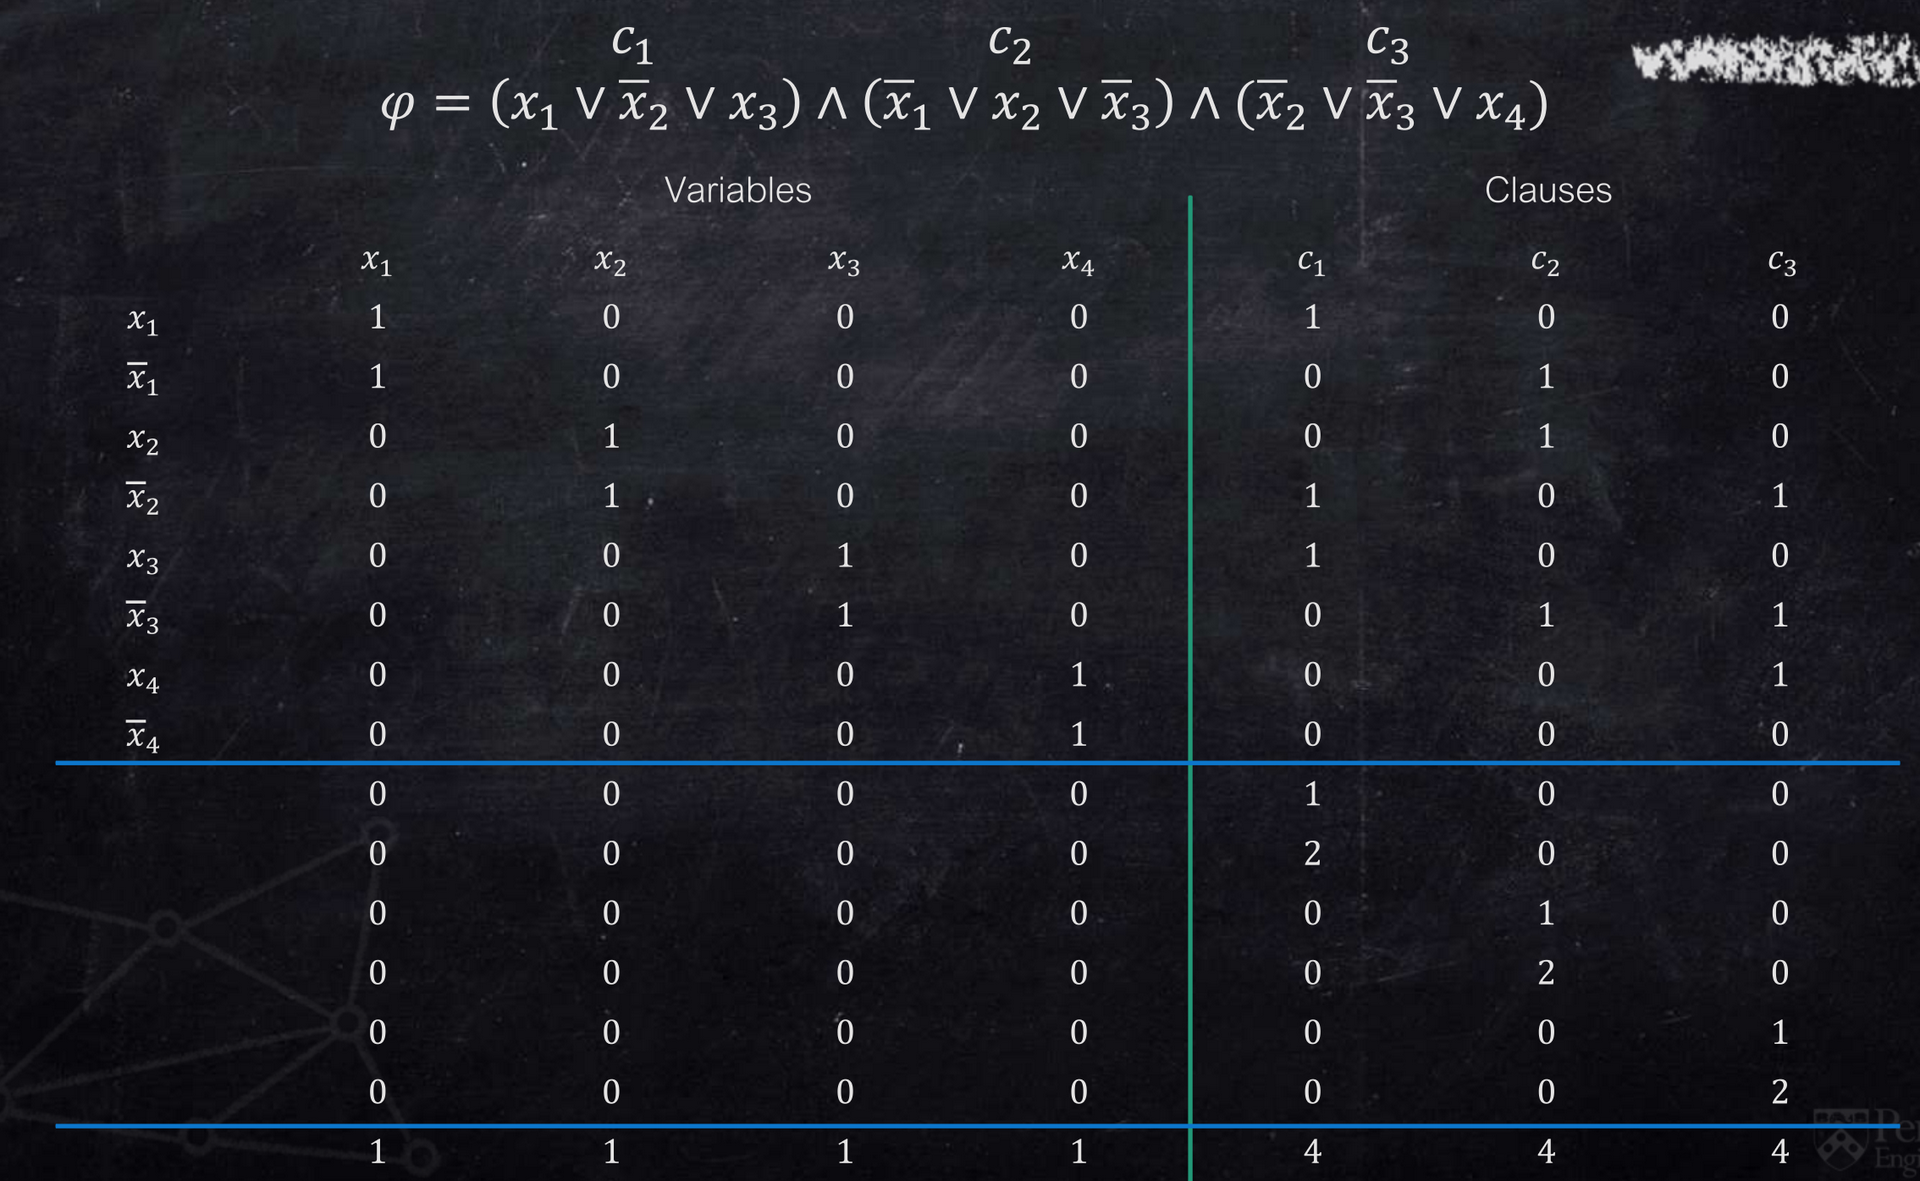
\includegraphics[width=0.5\textwidth]{fig/subset-sum.png}	
\end{figure}

In general,
\begin{figure}[H]
	\centering
	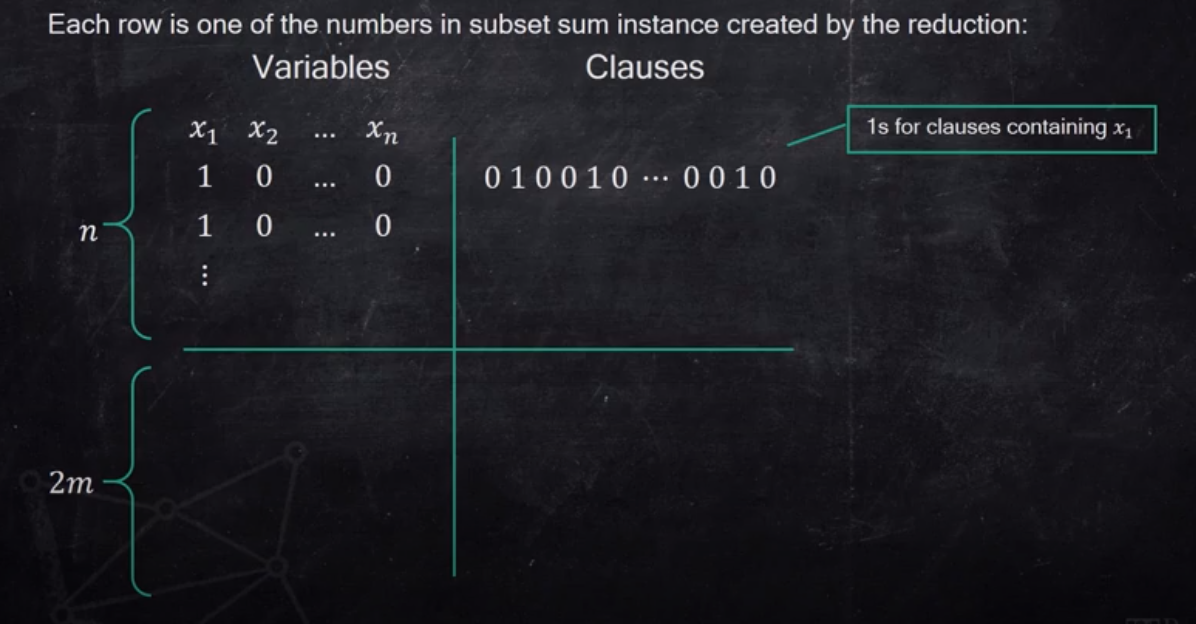
\includegraphics[width=0.5\textwidth]{fig/subset-sum-general.png}	
\end{figure}

\subsubsection{Proof of Correcness}
Suppose $\varphi$ is satisfiable. Let $a$ be a satisfying assignment for $\varphi$. Pick the numbers corresponding to the true literals in $a$. In the variable columns, we have picked one 1 per column, so the target is met. In any clause column, we have picked at least one 1 from the upper half but may have picked up to three 1s (if all 3 literals in the clause are true). Then we can get to the target of 4 by picking one or both numbers from lower half that have non-zero entries for that column. So, we have created a YES instance of subset sum.

If we have created a YES instance of subset-sum, look at the subset of numbers that add up to the target. Note that we only consider the YES-instance constructed by algorithm instead of any YES-instance.

For each variable $x_i$, this subset must have exactly one of the two numbers corresponding to $x_i$ or $(\bar{x_i})$. Treat the literal corresponding to the chosen number as TRUE. Then in each clause column, the chosen numbers (true literals) must contribute at least 1, otherwise we couldn't get to the target of 4 or these columns. Thus, the assignment we have constructed is a satisfying assignment for $\varphi$. Thus, $\varphi$ must be a YES instance of 3-SAT.
